\documentclass[xcolor=dvipsnames]{beamer}
\date{}
\title{GUI}
\author{Bernd Porr}
\begin{document}
\begin{frame}
\titlepage
\end{frame}




\begin{frame}[fragile]
  \frametitle{GUI: Introduction}

  \begin{enumerate}
  \item Old approach: XML for Layout, code for rest
  \item New approach: Everything is code
  \end{enumerate}
  
\end{frame}



\begin{frame}[fragile]
\frametitle{Example: Jackpack compose}
\begin{figure}[!hbt]
\begin{center}
\mbox{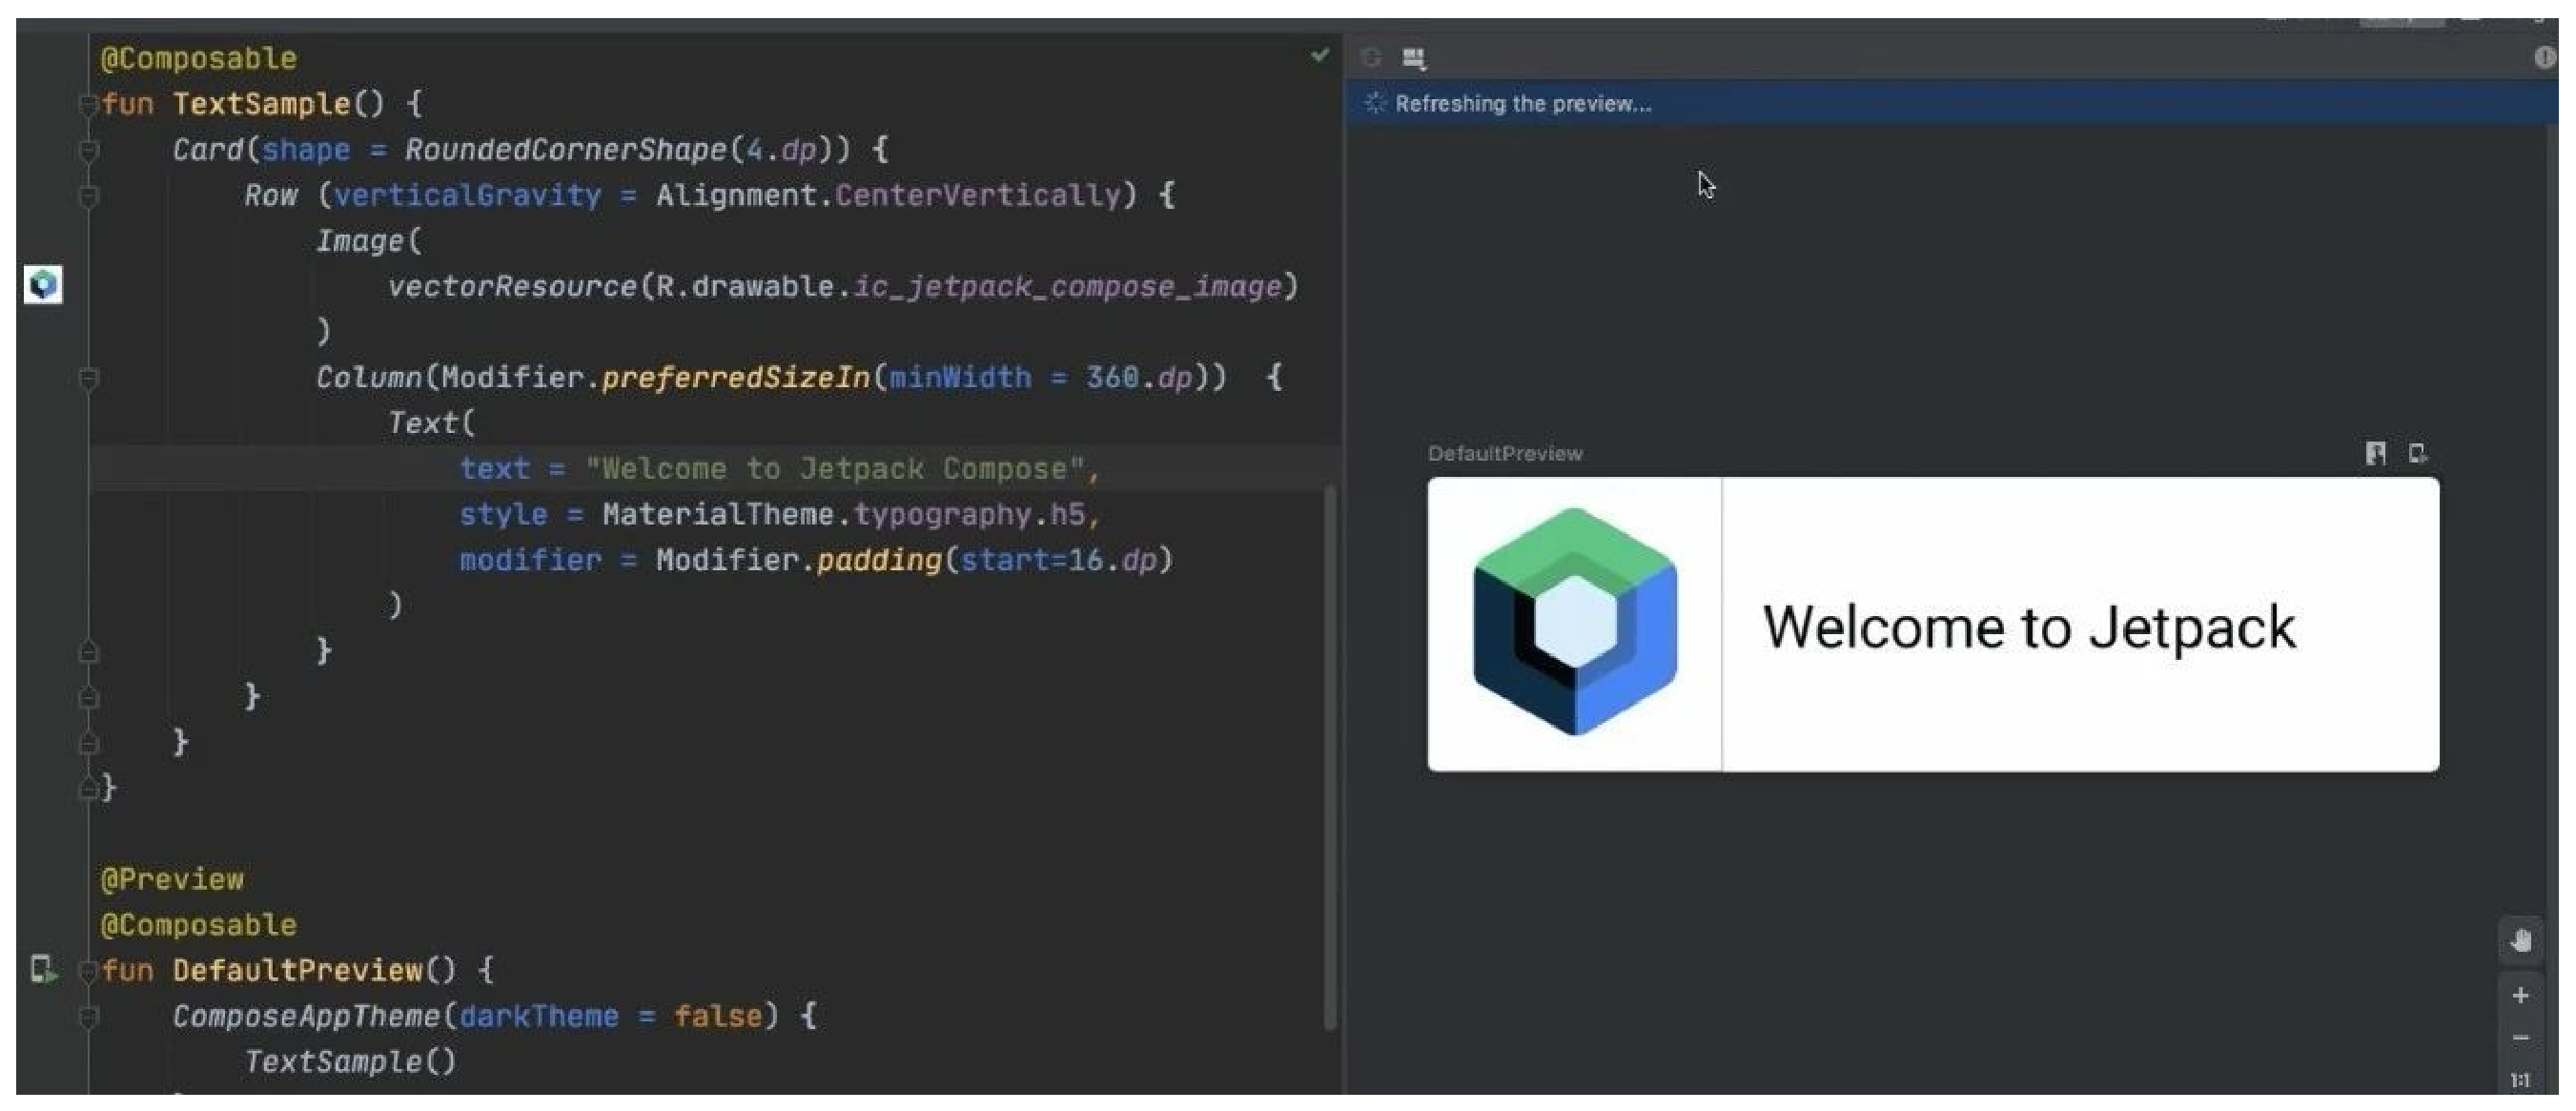
\includegraphics[width=\textwidth]{jetpack}}
\end{center}
\end{figure}
Definition of the layout with KOTLIN class instances.
\end{frame}



  
\begin{frame}[fragile]
  \frametitle{Example: SwiftUI}
\begin{figure}[!hbt]
\begin{center}
\mbox{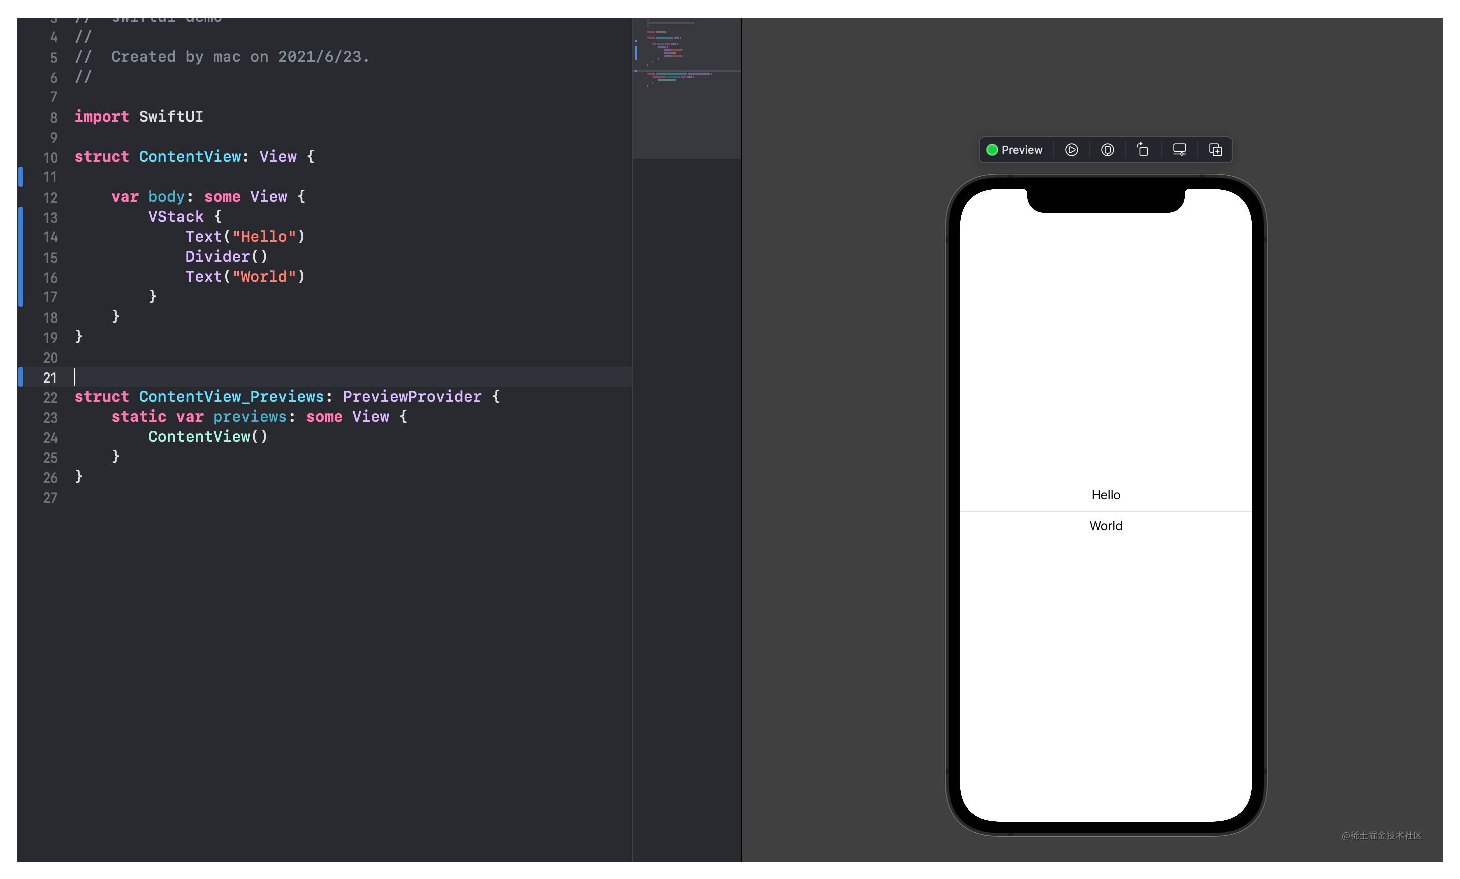
\includegraphics[width=\textwidth]{swiftui}}
\end{center}
\end{figure}
Again, definition of the layout with SWIFT class instances.
\end{frame}



  

\begin{frame}[fragile]
  \frametitle{QT}

  \begin{itemize}
\item \textbf{Qt} is a cross-platform windows development environment for
Linux, Windows and Mac written in C++.

\item Elements in Qt are \textsl{Widgets} which can contain anything form
  plots, buttons, text fields or the layout themselves. They are classes.
  
\item QT works with callbacks using a QT-specific signal/slot concept.
\end{itemize}
\end{frame}
  



\begin{frame}[fragile]
  \frametitle{Layout}

\begin{figure}[!hbt]
\begin{center}
\mbox{\includegraphics[width=0.5\textwidth]{qwtex}}
\end{center}
\caption{QT example layout
\label{qwtex}}
\end{figure}

Widgets are usually organised into
nested vertical and horizontal layouts
for the result). A lot of other options available.
\end{frame}



\begin{frame}[fragile]
  \frametitle{Layout II}

\begin{verbatim}
// create 3 widgets
button = new QPushButton;
thermo = new QwtThermo; 
plot = new QwtPlot;

// vertical layout
vLayout = new QVBoxLayout;
vLayout->addWidget(button);
vLayout->addWidget(thermo);

// horizontal layout
hLayout = new QHBoxLayout;
hLayout->addLayout(vLayout);
hLayout->addWidget(plot);

// main layout
setLayout(hLayout);
\end{verbatim}
\end{frame}



\begin{frame}[fragile]
\frametitle{Events from widgets}
A method of a class needs to be combined with the instance
pointer. The Qt method ``connect'' does exactly that:
\begin{verbatim}
connect(button, &QPushButton::clicked,
        this, &Window::reset);
\end{verbatim}
The QPushButton instance \texttt{button}
has a method called \texttt{clicked()} which is
called whenever the user clicks on the button.
This is then forwarded to the
method \texttt{reset()} in the application Widget.
\end{frame}


\begin{frame}[fragile]
\frametitle{Plotting realtime data arriving via a callback}
A callback \texttt{addSample()} is called in real-time whenever
a sample has arrived:
%should probably change memmove to std::move or whatever
\begin{verbatim}
void Window::addSample( float v ) {
    // add the new input to the plot
    std::move( yData, yData + plotDataSize - 1, yData+1 );
    curve->setSamples(xData, yData, plotDataSize);
    yData[0] = v;
    plot->replot(); // triggers replot but not now
}
\end{verbatim}
which stores the sample \texttt{v} in the shift buffer \texttt{yData}.
\end{frame}


\begin{frame}[fragile]
\frametitle{Plotting realtime data arriving via a callback}
Then the screen refresh (which is slow) is done at
a lower and unreliable rate:
\begin{verbatim}
void Window::timerEvent( QTimerEvent * )
{
    update(); // triggers the update of all Widgets
}
\end{verbatim}
\end{frame}


\begin{frame}[fragile]
\frametitle{the \texttt{paintEvent()} callback}
\texttt{update()} triggers a
paint event and then Qt calls the callback \texttt{paintEvent()}
``as soon as possible'' (which is to say, not in real-time) to repaint
the canvas of the widget:
\begin{verbatim}
void ScopeWindow::paintEvent(QPaintEvent *) {
        QPainter paint( this );

        paint.drawLine( ... )
}
\end{verbatim}
\end{frame}


\begin{frame}[fragile]
\frametitle{In Qt timing is not guaranteed}
Note that neither the timer callback nor the \texttt{update()} function
provide reliable realtime timing.
So Qt timers cannot be used to sample data but should
only be used for screen refresh and other non-time-critical
tasks.
\end{frame}



\begin{frame}[fragile]
\frametitle{\ldots but what about QML???}


\textbf{GUI in QML (javascript-ish) $\Leftrightarrow$ C++ application}

\bigskip

The problem is that QML needs to call C++ but we have two
very different languages.

\end{frame}


\begin{frame}[fragile]
\frametitle{\ldots but what about QML? Part 2}

QML:\\
\mbox{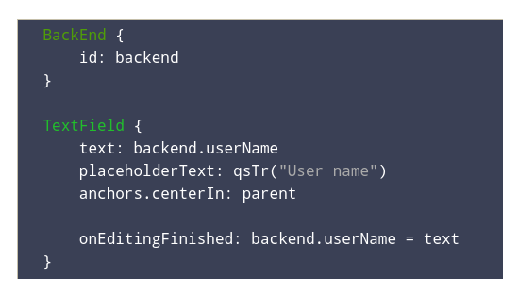
\includegraphics[width=0.5\textwidth]{qml_frontend}}

C++\\
\mbox{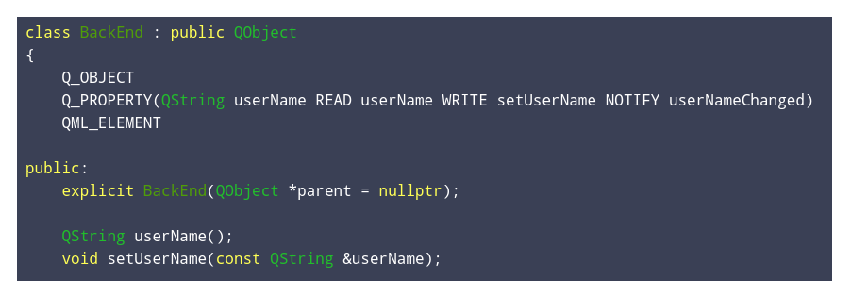
\includegraphics[width=\textwidth]{qml_backend}}


\end{frame}




\begin{frame}[fragile]
\frametitle{\ldots but what about QML? Part 3}

\mbox{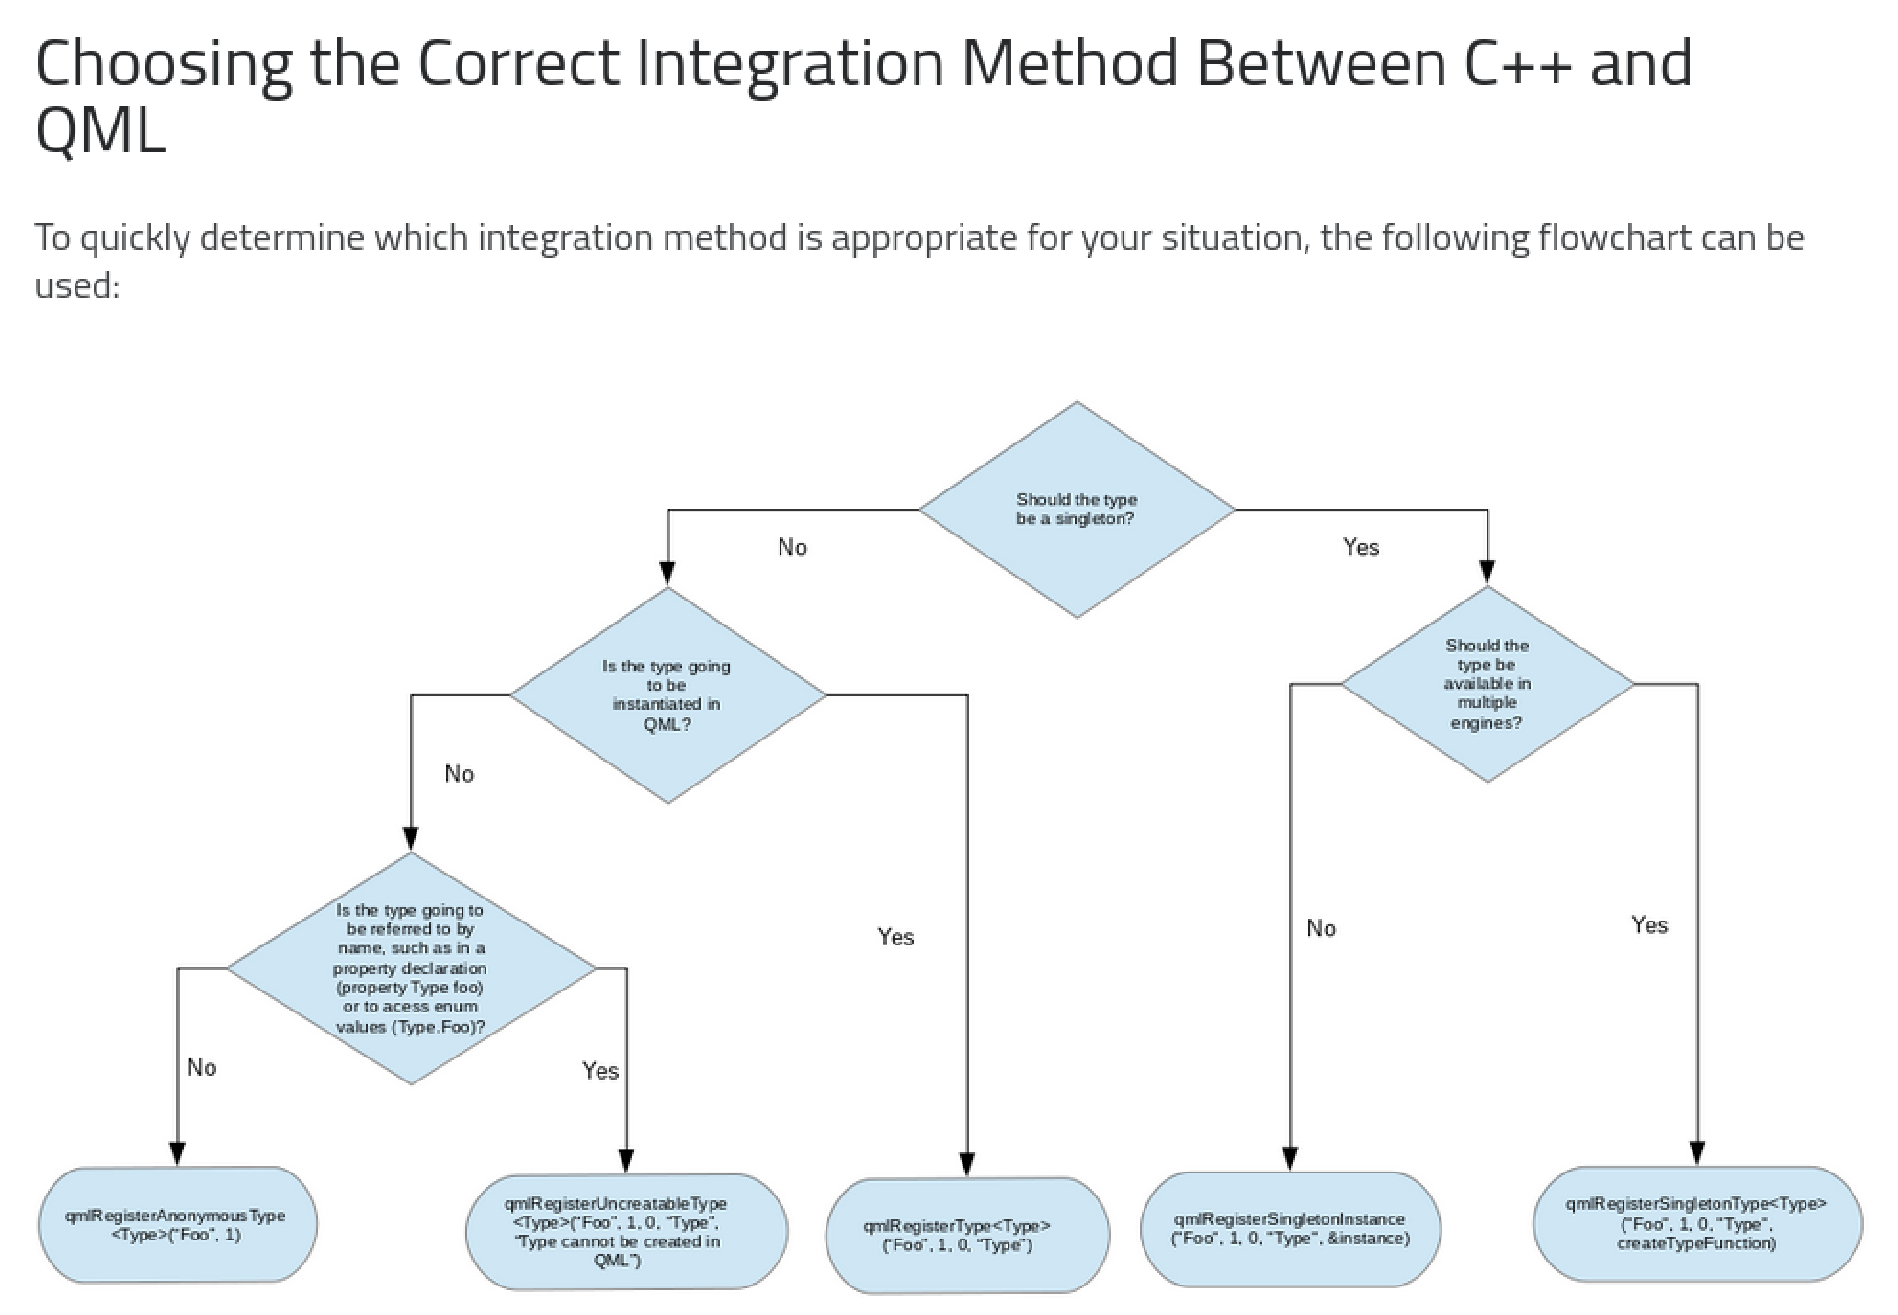
\includegraphics[width=\textwidth]{qml_choose}}

\mbox{
\includegraphics[width=0.1\textwidth]{emoj-dead}} \ldots so in a nutshell: don't do QML.

\end{frame}


\begin{frame}[fragile]
  \frametitle{GUI summary}

  Stick to C++ for \textsl{both} frontend (GUI) and backend.

  \bigskip

  Generally, the trend goes towards GUI- and backend in the
  \textsl{same language}.
\end{frame}



\end{document}
